\begin{figure}[tbp]
\centering
\begin{tikzpicture}[x=2.32cm,y=0.63cm,font=\small]
 \node[anchor=west] at (0,9.05) {(a) Constant fractional rates};
 
 \foreach \y/\rate/\job/\shade in {8.25/{3/4}/1/14,7.59/{1/2}/2/35,6.93/{1/2}/3/6}{
   \draw[fill=black!\shade] (0,\y) rectangle (2,{\y+.18});
   \node[anchor=west,inner sep=2pt] at (2,{\y+.09}) {$z_\job=\rate$};
 }
 \node[below,inner sep=1pt] at (0,6.79) {$0$};
 \node[below,inner sep=1pt] at (2,6.79) {$2$};
 \node[anchor=west] at (0,5.9) {(b) Row wrapping on the first half};
 \foreach \y/\mach in {4.95/1,4.22/2}{
   \draw (0,\y) rectangle (1,{\y+.48});
   \node[anchor=east] at (0,{\y+.24}) {$M_{\mach}$};
 }
 \draw[fill=black!14] (0,4.95) rectangle node {$1$} (.75,5.43);
 \draw[fill=black!35] (.75,4.95) rectangle node {$2$} (1,5.43);
 \draw[fill=black!35] (0,4.22) rectangle node {$2$} (.25,4.70);
 \draw[fill=black!6] (.25,4.22) rectangle node {$3$} (.75,4.70);
 \foreach \x/\labeltext in {0/0,.25/{\tfrac14},.75/{\tfrac34},1/1}{
   \draw (\x,4.08) -- (\x,3.94);
   \node[below] at (\x,3.94) {$\labeltext$};
 }
 \draw (0,4.01) -- (1,4.01);
 \node[anchor=west] at (0,2.84) {(c) First half and its reflection};
 \foreach \y/\mach in {1.95/1,1.22/2}{
  \draw (0,\y) rectangle (2,{\y+.48});
  \node[anchor=east] at (0,{\y+.24}) {$M_{\mach}$};
 }
 \draw[fill=black!14] (0,1.95) rectangle node {$1$} (.75,2.43);
 \draw[fill=black!35] (.75,1.95) rectangle node {$2$} (1,2.43);
 \draw[fill=black!35] (1,1.95) rectangle node {$2$} (1.25,2.43);
 \draw[fill=black!14] (1.25,1.95) rectangle node {$1$} (2,2.43);
 \draw[fill=black!35] (0,1.22) rectangle node {$2$} (.25,1.70);
 \draw[fill=black!6] (.25,1.22) rectangle node {$3$} (.75,1.70);
 \draw[fill=black!6] (1.25,1.22) rectangle node {$3$} (1.75,1.70);
 \draw[fill=black!35] (1.75,1.22) rectangle node {$2$} (2,1.70);
 \draw[densely dashed] (1,2.57) -- (1,1.10);
 \draw (0,1.01) -- (2,1.01);
 \foreach \x/\labeltext in {0/0,.25/{\tfrac14},.75/{\tfrac34},1/1,1.25/{\tfrac54},1.75/{\tfrac74},2/2}{
   \draw (\x,1.08) -- (\x,.94);
   \node[below] at (\x,.94) {$\labeltext$};
 }
\end{tikzpicture}
\caption{Reflected realization on two machines. The cells are labeled by job and blank cells are idle. Job~2 wraps between the two rows in the first half. Reflection about time~1 keeps each operation on its assigned machine.}\label[figure]{fig:reflection}
\end{figure}
